First, we seek to construct the explicit PWA representation of a ReLU network. Our method enumerates each polyhedral region and its associated affine map directly from the ReLU network. In Sec.~\ref{Cells} we show how polyhedra and affine maps are computed from the activation pattern of a ReLU network. In Sec.~\ref{Essential} we show how polyhedral representations are reduced to a minimal form, which is used in Sec.~\ref{Neighbors} to determine neighboring polyhedra given a current polyhedron. This leads to a recursive procedure, that we call Reachable Polyhedral Marching (RPM), in which we explore an expanding front of polyhedra, ultimately giving the explicit PWA representation, as explained in Sec.~\ref{Cell Enumeration}.

\subsection{Determining Polyhedral Regions from Activation Patterns} 
\label{Cells}

We show here that the network activation pattern $\blambda(\bx)$ from (\ref{Eq:AP}) has a one-to-one correspondence with the regions of the polyhedral tessellation underlying the ReLU network. We show how to explicitly extract the half-space constraints defining the polyhedron from the activation pattern. 

Consider the expression for the preactivation value $z_{ij}^{\text{pre}}$ in (\ref{Eq:PreActExplicit}). We can re-write this equation as
\begin{align}
\label{Eq:PreActHyperplane}
    z_{ij}^{\text{pre}} = [\bar\ba_{ij}^\top \quad  -\bar b_{ij}]\begin{bmatrix}
        \bx\\
        1
    \end{bmatrix},
\end{align}
where
\begin{align}
\label{Eq:HalfspaceDef}
    [\bar\ba_{ij}^\top \quad -\bar b_{ij}] = \boldsymbol{\theta}_{ij}\Big(\prod_{l = 1}^{i-1}\bLambda_{(l)}(\bx)\bTheta_l\Big).
\end{align} 
The activation $\lambda_{(ij)}$ is decided by the test $z_{ij}^\text{pre} > 0$, which we can write as $\bar\ba_{ij}^\top\bx > \bar b_{ij}$, defining a halfspace constraint in the input space.  Specifically, we have the following cases,
\begin{align}
\label{Eq:HalfspaceCases}
    \begin{cases}
          \bar\ba_{ij}^{\top} \bx > \bar b_{ij} \quad \text{if} \quad  \lambda_{(ij)} = 1 \\    
          \bar\ba_{ij}^{\top} \bx \le \bar b_{ij} \quad \text{if} \quad  \lambda_{(ij)} = 0.
      \end{cases}
\end{align}
This defines a halfspace constraint, that may or may not be open (due to the strict `$>$' inequality). However, on the boundary $\bar\ba_{ij}^\top\bx = \bar b_{ij}$, we have $z_{ij}^{\text{pre}} = 0$ from (\ref{Eq:PreActHyperplane}), leading to the post activation hidden state $z_{ij} = \lambda_{(ij)}z_{ij}^{\text{pre}} = 0$. We see that the value of the activation $\lambda_{(ij)}$ is irrelevant on the boundary, as the post activation state evaluates to zero regardless. We can therefore replace the `$>$' with `$\ge$' in (\ref{Eq:HalfspaceCases}) without loss of generality. 

% we  define $\ba_{ij} = -\bar\ba_{ij}/\|\bar\ba_{ij}\|$ and $b_{ij} = -\bar b_{ij}/\|\bar\ba_{ij}\|$ when $\lambda_{(ij)} = 1$, and $\ba_{ij} = \bar\ba_{ij}/\|\bar\ba_{ij}\|$ and $b_{ij} = \bar b_{ij}/\|\bar\ba_{ij}\|$ when $\lambda_{(ij)} = 0$. Or more succinctly,
Finally, to obtain the standard normalized form for a halfspace constraint ($\ba_{ij}^\top \bx \le b_{ij}$), we define
\begin{subequations}
\begin{align}
    \ba_{ij} &= (1-2\lambda_{(ij)})\frac{\bar\ba_{ij}}{\|\bar\ba_{ij}\|} \\
    b_{ij} &= (1-2\lambda_{(ij)})\frac{\bar b_{ij}}{\|\bar\ba_{ij}\|},
\end{align}
\label{eq:normalize}
\end{subequations}
where, in the degenerate case when $\bar\ba_{ij} = \mathbf{0}$, we define $\ba_{ij} = \mathbf{0}$ and $b_{ij} = \bar b_{ij}$. Hence, we obtain one halfspace constraint $\ba_{ij}^\top \bx \le b_{ij}$ for each neuron activation state $\lambda_{(ij)}$.

Given a specific input $\bx$, we can then take the resulting activation pattern of the network $\lambda(\bx)$, and directly extract the halfspace constraints that apply at that activation state from (\ref{Eq:HalfspaceCases}). In fact, (\ref{Eq:HalfspaceDef}) shows that $(\ba_{ij}, b_{ij})$ are actually functions of the activation patterns at earlier layers in the network. Indeed, consider perturbing $\bx$ as $\bx' = \bx + \boldsymbol{\delta}$. The halfspace constraints $(\ba_{ij}, b_{ij})$ will remain fixed under this perturbation until $\bdelta$ is large enough to change the activation pattern of an earlier layer $\lambda_{(l)}$, $l<i$. Consider the set of all such perturbed input values $\bx$ that do not result in a change in any neuron activation. We have
\begin{align}
    \label{eq:hrep_2}
    \scalemath{0.94}{P_{\lambda} = \{\bx \mid \ba_{ij}^\top \bx \le b_{ij} \quad i = 1, \ldots, L-1, \, j = 1, \ldots, l_i\}}, 
\end{align}
which is a polyhedron. We see that for each activation pattern $\lambda$, there exists an associated polyhedron $P$ in the input space over which that activation pattern remains constant. The procedure for determining the polyhedron associated with an activation pattern is formalized in Algorithm \ref{Algo:ap_to_poly}. A unique activation pattern $\lambda_k$ can then be defined for each affine region $k$. To be clear, we refer to the activation pattern for region $k$ as $\lambda_k$, and use subscripts in parentheses to refer to the specific layer and neuron activation values. Lastly, for a fixed activation pattern, from (\ref{Eq:NNExplicit}) the ReLU network simplifies to the affine map $\by = \mathbf{C}_k \bx + \mathbf{d}_k$ where
\begin{align}
\label{eq:CdDef}
    \begin{bmatrix}
        \bC_k & \bd_k
    \end{bmatrix} &= 
    \bTheta_L\Big(\prod_{i = 1}^{L-1}\bLambda_{k,(i)}(\bx)\bTheta_i\Big).
\end{align}

\begin{algorithm}[h!]
\setlength\belowcaptionskip{-0.5\baselineskip}
\SetAlgoLined
\DontPrintSemicolon
 \KwIn{$\lambda$}
 \KwOut{$\bA, \bb$}
 $k \leftarrow 1$ \\
\For{$i = 1,\ldots,L-1$, $j = 1,\ldots,l_i$}{
$\Bar{\mathbf{a}}_{ij},\ \Bar{b}_{ij} \leftarrow$ (\ref{Eq:HalfspaceDef}) \\
$\mathbf{a}_{ij},\ b_{ij} \leftarrow$ (\ref{eq:normalize}) \\
$\bA[k,:],\ \bb[k] \leftarrow \mathbf{a}_{ij},\ b_{ij}$ \\
$k \leftarrow k+1$
}
\Return{$\bA, \bb$}
\caption{Polyhedron from Activation Pattern}
\label{Algo:ap_to_poly}
\end{algorithm}

%The activation pattern only changes if some $\hat{z}_{ij}$ switches from positive to nonpositive (or vice-versa). The region $P$ is thus given by a set of linear constraints, one for each neuron in the network.  The constraint for neuron $j$ in layer $i$ is

%where
%\begin{align}
%    \begin{bmatrix}
%        \mathbf{a}_{ij} & -b_{ij}
%    \end{bmatrix} =  
%    \tilde{\mathbf{W}}_i[j,:] \prod_{l=1}^{i-1} \tilde{\mathbf{W}}_l^P, \label{eq:ab}
%\end{align}
%and $\tilde{\mathbf{W}}_i[j,:]$ denotes the $j^{th}$ row of $\tilde{\mathbf{W}}_i$. Equation (\ref{eq:ab}) is similar to (\ref{eq:linear}) but instead simply gives the affine map parameters for a single neuron output. Strict inequalities are not present in (\ref{eq:constraints}) because the affine map $\by = \mathbf{C}^P\bx + \mathbf{d}^P$ holds over the interior and boundary of the set where the activation pattern is constant. Since $P$ is an intersection of halfspaces, the set is a polyhedron. A similar formulation is given in \cite{lei2020analytic} for finding the surface of an object for graphics rendering. Note that it is common for neurons to elicit the degenerate linear constraint $\mathbf{0}^{\top} \bx \le b$ for some $b \ge 0$, which is trivially satisfied for all $\bx \in P$. In addition, different neurons in the network can define equivalent constraints (perhaps scaled arbitrarily). To address these edge cases we introduce Definitions  \ref{def: normalize}, \ref{def: duplicate}, \ref{def: redundant} before describing our algorithm.  

% \begin{definition}[H-representation]
% The halfspace representation (H-representation) of a polyhedron is  
% \begin{align}
%     P_H = \{\bx \in \mathbb{R}^d \mid \mathbf{A} \bx \le \mathbf{b} \} \label{eq:hrep}
% \end{align}
% where $\mathbf{A}$ an $m \times d$ matrix and $\mathbf{b}$ an $m$-dimensional vector. Equality constraints may also be included if the set $P_H$ is of lower dimension than the ambient dimension. \label{def: hrep}
% \end{definition}

%\begin{definition}[Normalized Constraints]
%We can define a normalized constraint for the hyperplane $[\mathbf{a}_{ij} \ \ b_{ij}]$ associated with neuron $ij$ by defining
%\begin{subequations}
%\begin{align}
%    \tilde{\mathbf{a}}_{ij} &= (1-2AP_{ij})\frac{\mathbf{a}_{ij}}{\vert \vert \mathbf{a}_{ij} \vert \vert _2} \\
%    \tilde{b}_{ij} &= (1-2AP_{ij})\frac{b_{ij}}{\vert \vert \mathbf{a}_{ij} \vert \vert _2}
%\end{align}
%\label{eq:normalize}
%\end{subequations}
%In the case $\mathbf{a}_{ij} = \mathbf{0}$, then $\tilde{\mathbf{a}}_{ij} = \mathbf{0}$ and $\tilde{b}_{ij} = b_{ij}$. By performing this normalization we ensure that $\tilde{\mathbf{a}}_{ij}^{\top} \bx \le \tilde{b}_{ij}$ is valid given $AP_{ij}$ \label{def: normalize}
%\end{definition}

%%%%%%%%%%%%%%%%%%%%%%%%%%%%%%%%%%%%
\subsection{Finding Essential Constraints} \label{Essential}
%%%%%%%%%%%%%%%%%%%%%%%%%%%
As mentioned previously, a polyhedron may have redundant constraints. We find that many of the constraints for the polyhedron $P_k$ generated by $\lambda_k$ are either duplicates or redundant, and can thus be removed. We define more formally the concepts of duplicate and redundant constraints.
\begin{definition}[Duplicate Constraints]
A constraint $\mathbf{a}_j^{\top} \bx \le b_j$ is duplicate if there exists a scalar $\alpha > 0$ and a constraint $\mathbf{a}_i^{\top} \bx \le b_i$, $i<j$, such that $\alpha [\mathbf{a}^\top_j\ b_j] = [\mathbf{a}^\top_i\ b_i]$. \label{def: duplicate}
\end{definition}
\begin{definition}[Redundant \& Essential Constraints]
A constraint is redundant if the feasible set does not change upon its removal. An essential constraint is not redundant. \label{def: redundant}
\end{definition}

We next describe how to remove the redundant constraints in a H-representation, leaving only the essential halfspace constraints. We first normalize all constraints, remove any duplicate constraints, and consider the resulting  H-representation $\mathbf{A}\bx \le \mathbf{b}$. To determine if the remaining $i^{\text{th}}$ constraint is essential or redundant, we define a new set of constraints with the $i^{\text{th}}$ constraint removed,
\begin{subequations}
    \label{eq:pre-LP}
    \begin{align}
        \tilde{\mathbf{A}} = [\mathbf{a}_1 \ldots \mathbf{a}_{i-1}\ \mathbf{a}_{i+1} \ldots \mathbf{a}_M]^\top \\
         \tilde{\mathbf{b}} = [b_1 \ldots b_{i-1}\ b_{i+1} \ldots b_M]^\top,
    \end{align}
\end{subequations}
and solve the linear program
\begin{subequations}
    \label{eq:LP}
    \begin{align}
        \max_{\bx} \quad & \mathbf{a}^{\top}_i \bx\\
        \textrm{subject to} \quad & \tilde{\mathbf{A}}\bx \le \tilde{\mathbf{b}}.
    \end{align}
\end{subequations}
If the optimal objective value is less than or equal to $b_i$, constraint $i$ is redundant. 
Note, it is critical that any duplicate constraints are removed before this procedure. We formalize this procedure in Algorithm \ref{Algo:essential hrep}.
\begin{algorithm}[h!]
\SetAlgoLined
\DontPrintSemicolon
 \KwIn{$\lambda$}
 \KwOut{$\bA, \bb$}
 $\bA, \bb \leftarrow$ Algorithm \ref{Algo:ap_to_poly} \\
 $\bA, \bb \leftarrow$ remove duplicate constraints of $\bA, \bb$  \\
 $\tilde{\bA}, \tilde{\bb} \leftarrow$ $\bA, \bb$ \algorithmiccomment{make copy of $\bA, \bb$} \\
\For{$\ba_i, b_i \in \bA, \bb$}{
$\tilde{\bA}, \tilde{\bb} \leftarrow$ remove $\ba_i, b_i$ from $\tilde{\bA}, \tilde{\bb}$ \\
$p^* \leftarrow$ optimal objective value of (\ref{eq:LP})  \\
\If{$p^* > b_i$}
{add $\ba_i, b_i$ back to $\tilde{\bA}, \tilde{\bb}$}

}
$\bA, \bb \leftarrow \tilde{\bA}, \tilde{\bb}$ \\
\Return{$\bA, \bb$}
\caption{Essential H-representation}
\label{Algo:essential hrep}
\end{algorithm}

In the worst case, a single LP must be solved for each constraint to determine whether it is essential or redundant. However, heuristics exist to practically avoid this worst case complexity. For computational efficiency, Algorithm \ref{Algo:essential hrep} can be modified to first identify and remove a subset of redundant constraints using the bounding box heuristic \cite{morari}. We observe that this can result in identifying as many as $90\%$ of the redundant constraints. We find that other heuristics such as ray-shooting do not improve performance in our tests.



% One additional performance increase is taken advantage of when solving for essential constraints. The LPs for each constraint check are very similar and many solvers will experience speedup when the problem is edited instead of reinstantiated for each constraint query. The effect of this is significant, and empirically leads to enumerating essential constraints nearly twice as fast compared to reinstantiating the LP for each constraint. We use the GLPK open-source LP solver and the JuMP optimization package \cite{DunningHuchetteLubin2017} to solve LPs.

%%%%%%%%%%%%%%%%%%%%%%%%%%%%%%%%%%%%%%%%%%%%%%%%%%
%%%%%%%%%%%%%%%%%%%%%%%%%%%%%%%%%%%%%%%%%%%%%%%%%%
\begin{figure*}[t]
    \setlength\belowcaptionskip{-0.5\baselineskip}
     \centering
     \begin{subfigure}[b]{0.24\textwidth}
         \centering
         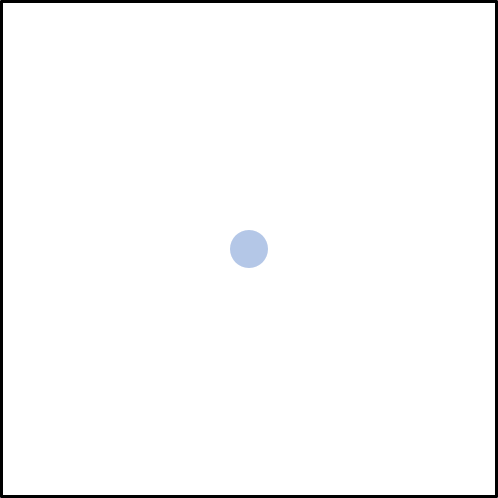
\includegraphics[width=\textwidth]{figs/rpm_1.png}
         \caption{}
     \end{subfigure}
     \hfill
     \begin{subfigure}[b]{0.24\textwidth}
         \centering
         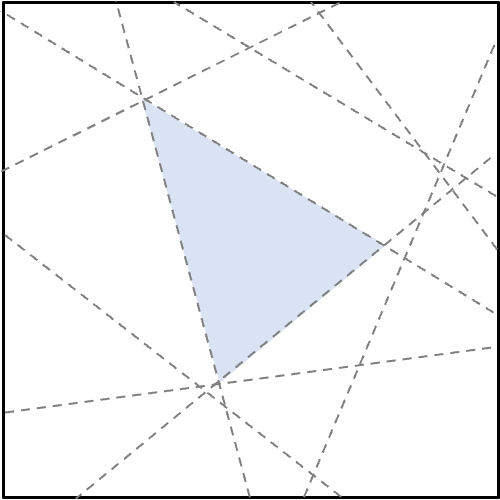
\includegraphics[width=\textwidth]{figs/rpm_2.png}
         \caption{}
     \end{subfigure}
     \hfill
     \begin{subfigure}[b]{0.24\textwidth}
         \centering
         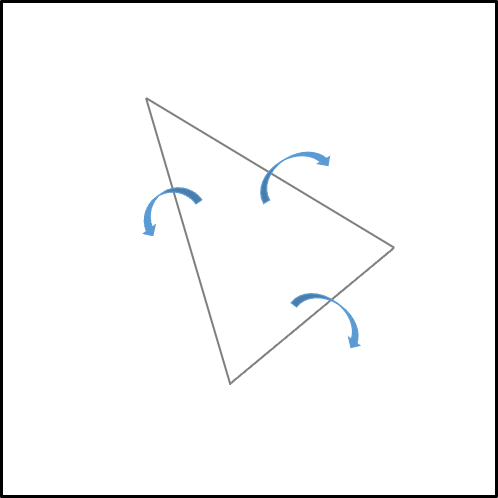
\includegraphics[width=\textwidth]{figs/rpm_3.png}
         \caption{}
     \end{subfigure}
     \hfill
     \begin{subfigure}[b]{0.24\textwidth}
         \centering
         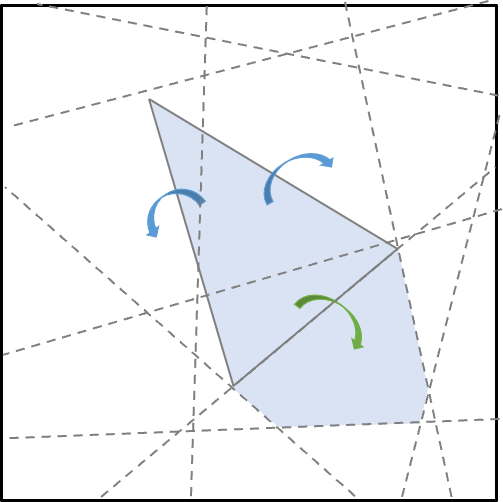
\includegraphics[width=\textwidth]{figs/rpm_4.png}
         \caption{}
     \end{subfigure}
        \caption{This figure illustrates the main steps of the RPM algorithm (Algorithm \ref{Algo:cell_enumeration}). (a) The algorithm is initialized with a point in the input space that is evaluated by the ReLU network to determine the activation pattern $\lambda$. (b) Then the polyhedron corresponding to $\lambda$ is computed using Algorithm \ref{Algo:ap_to_poly}. (c) Next, the essential constraints for the polyhedron, which in turn connect it to unexplored neighboring regions (indicated by blue arrows), are determined using Algorithm \ref{Algo:essential hrep}. (d) Then the activation pattern for a neighboring region (indicated by the green arrow) is found using Algorithm \ref{Algo:neighbor_ap}. The process then repeats by recursively exploring neighboring regions in this manner until the entire input set is explored.}
        \label{fig:alg_steps}
\end{figure*}

\subsection{Determining Neighboring Activation Patterns} \label{Neighbors}
Consider two neighboring polyhedra $P_k$ and $P_{k'}$ such that their shared face is identified by $\ba_\eta^\top \bx = b_\eta$ and $\ba_\eta^\top \bx \le b_\eta$ is an essential constraint for $P_k$, while $-\ba_\eta^\top \bx \le -b_\eta$ is an essential constraint for $P_{k'}$. We call $\ba_\eta^\top \bx \le b_\eta$ the neighbor constraint. Given the neuron activation pattern $\lambda$ for $P_k$, we next describe a procedure to find the activation pattern $\lambda'$ for $P_{k'}$, from which we can find the essential halfspace constraints from the procedure described in the previous section. This allows us to systematically generate all the activation patterns that are realizable by the network, and to obtain the polyhedra and affine maps associated with each of those activation patterns.  

Intuitively, to generate $\lambda_{k'}$ one ought to simply flip the activation of the neurons defining $\ba_\eta^\top \bx \le b_\eta$, and compute all the resulting new halfspace constraints from later layers in the network from (\ref{Eq:HalfspaceDef}). However, this intuitive procedure is incomplete because it does not correctly account for the influence that one neuron may have on other neurons in later layers. Flipping one neuron may lead to other neurons in later layers being flipped as well. To correctly determine the downstream effects of flipping a neuron, we provide a theorem for when neuron activations must be flipped.

\begin{theorem}[Neighboring Activation Patterns]
\label{thm: activation_flipping}
For a given region $P_k$, each neuron defines a hyperplane $\ba_{k,ij}^\top \bx = b_{k,ij}$, as given by (\ref{eq:normalize}). Suppose regions $P_k$ and $P_{k'}$ neighbor each other and are separated by $\ba_\eta^\top \bx = b_\eta$ where $P_{k} \subset \{\bx \mid \ba_\eta^\top \bx \le b_\eta \}$. Then,
\begin{enumerate}
    \item if $[\ba_{k,ij}^\top\quad  -b_{k,ij}] \neq \alpha[\ba_\eta^\top\quad -b_\eta]$ for some $\alpha \in \{0,1\}$, the activation of neuron $ij$ does not change, $\lambda_{k,ij} = \lambda_{k',ij}$.
    \item If $[\ba_{k,ij}^\top\quad  -b_{k,ij}] = \alpha[\ba_\eta^\top\quad -b_\eta]$ for some $\alpha \in \{0,1\}$, then $[\ba_{k',ij}^\top\quad  -b_{k',ij}] = \alpha[\ba_\eta^\top\quad -b_\eta]$ for some $\alpha \in \{-1,0\}$, and the activation $\lambda_{k',ij}$ should be set to ensure this holds.
\end{enumerate}
\end{theorem}

The proof for Theorem \ref{thm: activation_flipping} is in the Appendix. Then, the procedure to generate a neighboring activation pattern is defined in Algorithm \ref{Algo:neighbor_ap}. We present Algorithm \ref{Algo:neighbor_ap} in as simple a manner as possible, however, for a more efficient approach, one need not loop over all neurons in the network, but only those that meet condition 2) of Theorem \ref{thm: activation_flipping}.

% \begin{definition}[Type 1, 2, 3 neurons] \label{types}
% \textcolor{black}{Mac: Not formal enough, I think.  Let's discuss.} When identifying the activation pattern $\lambda'$ for a neighboring region $P'$ from a current region $P$, neurons whose halfspace constraints in $P$ define a non-empty boundary $P \cap P'$ are called \textit{Type 1}. Neurons with degenerate halfspace constraints in $P$, $\mathbf{0}^{\top} \bx \le b \ \forall \bx \in P$ where $b\ge 0$ are called \textit{Type 2}. All other neurons are \textit{Type 3}. 
% \end{definition}

% We find, in fact, that when flipping a neuron $\lambda_{(ij)}$ only Type 1 and Type 2 neurons in later layers $\lambbda_{kl}$, $k>i$, may be flipped as a result, according to the rules in the following theorem. \textcolor{black}{Mac: We need a formal theorem here, which is proved in the proof in the appendix.} 




\begin{algorithm}[!h]
\SetAlgoLined
\DontPrintSemicolon
 \KwIn{$\lambda_k$, $\mathbf{a}_\eta$, $b_\eta$, $\bTheta$}
 \KwOut{$\lambda_{k'}$}
 $\lambda_{k'} \leftarrow  \lambda_k$ \algorithmiccomment{Initialize neighbor region $\lambda$} \\
 
\For{$i = 1,\ldots,L-1$, $j = 1,\ldots,l_i$}{ 
% $\mathbf{a}_{ij},\ b_{ij} \leftarrow$ Equation \ref{eq:ab} \algorithmiccomment{$\lambda_{k',ij}$ hyperplane} \\
$\mathbf{a}_{k',ij},\ b_{k',ij} \leftarrow$ (\ref{eq:normalize}) \\
\uIf{$\mathbf{a}_{k',ij} = \mathbf{a}_\eta \quad \textbf{\upshape and}\quad b_{k',ij} = b_\eta$}
{$\lambda_{k',ij} \leftarrow \neg \lambda_{k,ij} $}
\uElseIf{$\mathbf{a}_{k',ij} = \mathbf{0} \quad \textbf{\upshape and}\quad b_{k',ij} = 0$}
{$\lambda_{k',ij} \leftarrow 0$}
}
\Return{$\lambda_{k'}$}
\caption{Neighboring Activation Pattern}
\label{Algo:neighbor_ap}
\end{algorithm}

% \begin{algorithm}[!h]
% \SetAlgoLined
% \DontPrintSemicolon
%  \KwIn{$\lambda_k$, $\mathbf{a}_\eta$, $b_\eta$, $\Theta$}
%  \KwOut{$\lambda_{k'}$}
%  $\lambda_{k'} \leftarrow  \lambda_k$ \algorithmiccomment{Initialize new $\lambda$ as old $\lambda$} \\
 
% \For{$i \in [1,\ldots,n-1]$, $j \in [1,\ldots,l_i]$}{ 
% \If{$ij \in$ \upshape Type 1  or $ij \in$ \upshape Type 2}{
% % $\mathbf{a}_{ij},\ b_{ij} \leftarrow$ Equation \ref{eq:ab} \algorithmiccomment{$\lambda_{k',ij}$ hyperplane} \\
% $\mathbf{a}_{ij},\ b_{ij} \leftarrow$ Equation \ref{eq:normalize} \\
% \uIf{$\mathbf{a}_{ij} = \mathbf{0} \quad \textbf{\upshape and}\quad b_{ij} < 0$}
% {$\lambda_{k',ij} \leftarrow \neg \lambda_{k,ij} $}
% \uElseIf{$\mathbf{a}_{ij} = \mathbf{a}_\eta \quad \textbf{\upshape and}\quad b_{ij} < b_\eta$}{$\lambda_{k',ij} \leftarrow \neg \lambda_{k,ij} $}
% \ElseIf{$\mathbf{a}_{ij} = -\mathbf{a}_\eta \quad \textbf{\upshape and}\quad b_{ij} < -b_\eta$}{$\lambda_{k',ij} \leftarrow \neg \lambda_{k,ij} $}
% }
% }
 
% \Return{$\lambda_{k'}$}
% \caption{Neighboring Activation Pattern}
% \label{Algo:neighbor_ap}
% \end{algorithm}

% where the preactivation value of a neuron as a function of the input is 
% \begin{align}
%     \hat{z}_{ij}(\bx) = \mathbf{W}_i \mathbf{z}_{i-1}(\bx) + \mathbf{b}_i.
% \end{align}
% The closure of the feasible set given by all such nonlinear constraints is the polyhedron $c$. Finding which neuron activations to flip when $\bx$ transitions from $c$ to $c'$ is equivalent to finding which nonlinear constraints must be flipped such that the resulting feasible set is $c'$. The distinction between the linear constraints given by (\ref{eq:constraints}) and the nonlinear constraints given by (\ref{eq:nonlinear}) is that the nonlinear constraint equations $\hat{z}_{ij}(\bx)$ hold for all inputs $\bx \in \mathbb{R}^{k_0}$, whereas the linear constraint parameters $\mathbf{a}_{ij}$ and $b_{ij}$ are valid only for $\bx \in c$. \textcolor{black}{mac: The above explanation is too vague to be useful.  How are they mathematically related  What is equal to what and under what conditions?  Best to just find a better notation that only uses $a_{ij}$.} 

% the set of points where a nonlinear constraint equation equals zero is restricted to hyperplanes, when in fact a nonlinear constraint equation can equal zero over full dimensional sets as well. This is illustrated by neurons associated with the degenerate linear constraint $\mathbf{0}\cdot \bx = 0 \ \forall \bx \in c$. 

% Informally, flipping the sense of a nonlinear constraint flips which side of the constraint boundary is feasible. We seek to flip the sense of nonlinear constraints if doing so leads to feasibility in the $c'$. 
% The feasible set given by the intersection of each hidden neuron nonlinear constraint is exactly the polyhedron given by Equation (\ref{eq:constraints}). Moreover, the nonlinear constraints defined by an activation pattern are equivalent to the linear constraints from Equation (\ref{eq:constraints}) for $\bx \in c$. 
% Given the activation pattern of a ReLU network, neurons are associated with linear constraints by (\ref{eq:constraints}). These constraints are local in the sense that they are only valid for $\bx \in c$. But more generally, an activation pattern describes nonlinear constraints that hold for all inputs. For neuron $j$ in layer $i$
% \begin{align}
% \begin{cases}
% \hat{z}_{i,j}(\bx) \ge 0\ \ \text{if}\   \ AP_{i,j} = 1 \\
% \hat{z}_{i,j}(\bx) \le 0\ \ \text{if}\   \ AP_{i,j} = 0
% \end{cases}.
%  \label{eq:nonlinear}
% \end{align}
% For example, a nonlinear constraint in layer two is
% \begin{align}
% \hat{z}_{2,j}(\bx) =
% \begin{cases}
% \tilde{\mathbf{W}}_2[j,:]\sigma(\tilde{\mathbf{W}}_1 \tilde{\bx}) \ge 0 \ \ AP_{i,j} = 1 \\
%  \tilde{\mathbf{W}}_2[j,:]\sigma(\tilde{\mathbf{W}}_1 \tilde{\bx}) \le 0 \ \ AP_{i,j} = 0.
% \end{cases}
% \end{align}

% A nonlinear constraint is active when $\hat{z}_{i,j}(\bx) = 0$. Note that this is different than the notion of a ReLU being active or inactive. The region for which a nonlinear constraint is active is not restricted to be a lower dimensional facet of a cell. For instance Type 2 constraints are active over an entire cell.

% Since interior inputs from the original cell should be infeasible for the neighbor cell constraints, a naive approach to determining the neighboring activation pattern is to simply flip the neuron activation for each Type 1 neuron. This is the right intuition, but an incomplete approach. The intuition this draws on is that the sense of a nonlinear constraint should be flipped if the constraint boundary is coincident with the shared boundary between the original and neighbor cell. 

% Since we want to flip the sense of a nonlinear constraint if its constraint boundary is coincident with the shared neighbor boundary, it is useful to characterize where the constraints are active. 

% In addition, we must not flip the sense of nonlinear constraints associated with Type 2 neurons. Lastly, we may need to flip the sense of some constraints associated with Type 3 neurons.

% Equation \ref{g1} is true by construction of the Type 1 set. If Equation \ref{g2} were not true that would imply that the associated halfspace constraint for a Type 2 neuron would be equal to the halfspace constraint for a Type 1 neuron which is a contradiction according to the construction of the Type 1 and Type 2 sets. Thus Equation \ref{g2} is true. Equation \ref{g3} is true because the degenerate halfspace constraints associated with these neurons indicate that Type 3 neurons always evaluate to 0 on the parent cell (of which the shared boundary is included).

% \begin{enumerate}
%   \item If the updated linear constraint generated by a Type 1 neuron is $\mathbf{0} \cdot \bx \le 0$, then the updated activation for that neuron is $0$ (regardless of whether it was 1 or 0 in the original cell) (Figure \ref{fig:constraints}c). Otherwise, the activation is flipped (Figure \ref{fig:constraints}b).
%   \item If the updated linear constraint generated by a Type 2 neuron is equal and opposite to the original essential constraint (defined by Type 1 neurons), then the activation is flipped from a 0 to a 1 (Figure \ref{fig:constraints}d). Otherwise, it remains 0 (Figure \ref{fig:constraints}e).
% \end{enumerate}
% Note that since linear constraints are unchanged when multiplied by a scalar, the linear constraints from (\ref{eq:constraints}) must be normalized to perform the comparison in rule 2.

% We know that Type 1 nonlinear constraints are active at the boundary. Once past the boundary into the neighbor cell, these constraints can become inactive, in which case the sense of the constraint is flipped. Or they can remain active, in which case the constraint is not flipped. This corresponds to the constraint being active over the entire neighbor cell, and thus the neuron is a Type 3 neuron for the neighbor cell.

% Also, we know there exists some $\delta$ we can go past the shared boundary, into the neighbor cell, where the sense of the Type 2 nonlinear constrains do not flip. This is because each $g_{ij}(x)$ is a continuous function. Thus, the sense of Type 2 constraints remains the same.

% Like the Type 1 constraints, the constraint boundary for Type 3 neurons may lie coincident with the shared boundary. If coincident with the shared boundary, we must flip the sense of the nonlinear constraint. Otherwise we do not flip, as the original constraint is still active. Thus, the sense of a Type 3 nonlinear constraint will flip if and only if flipping the new halfspace constraint associated with it (after flipping necessary neurons in previous layers and re-computing the halfspace constraints) equals the new, flipped, Type 1 constraints.


%%%%%%%%%%%%%%%%%%%%%%%%%%%%%%%%%%%%%%%%%%%%%%%%%%
%%%%%%%%%%%%%%%%%%%%%%%%%%%%%%%%%%%%%%%%%%%%%%%%%%
\subsection{Reachable Polyhedral Marching} \label{Cell Enumeration}
% \begin{figure*}
%     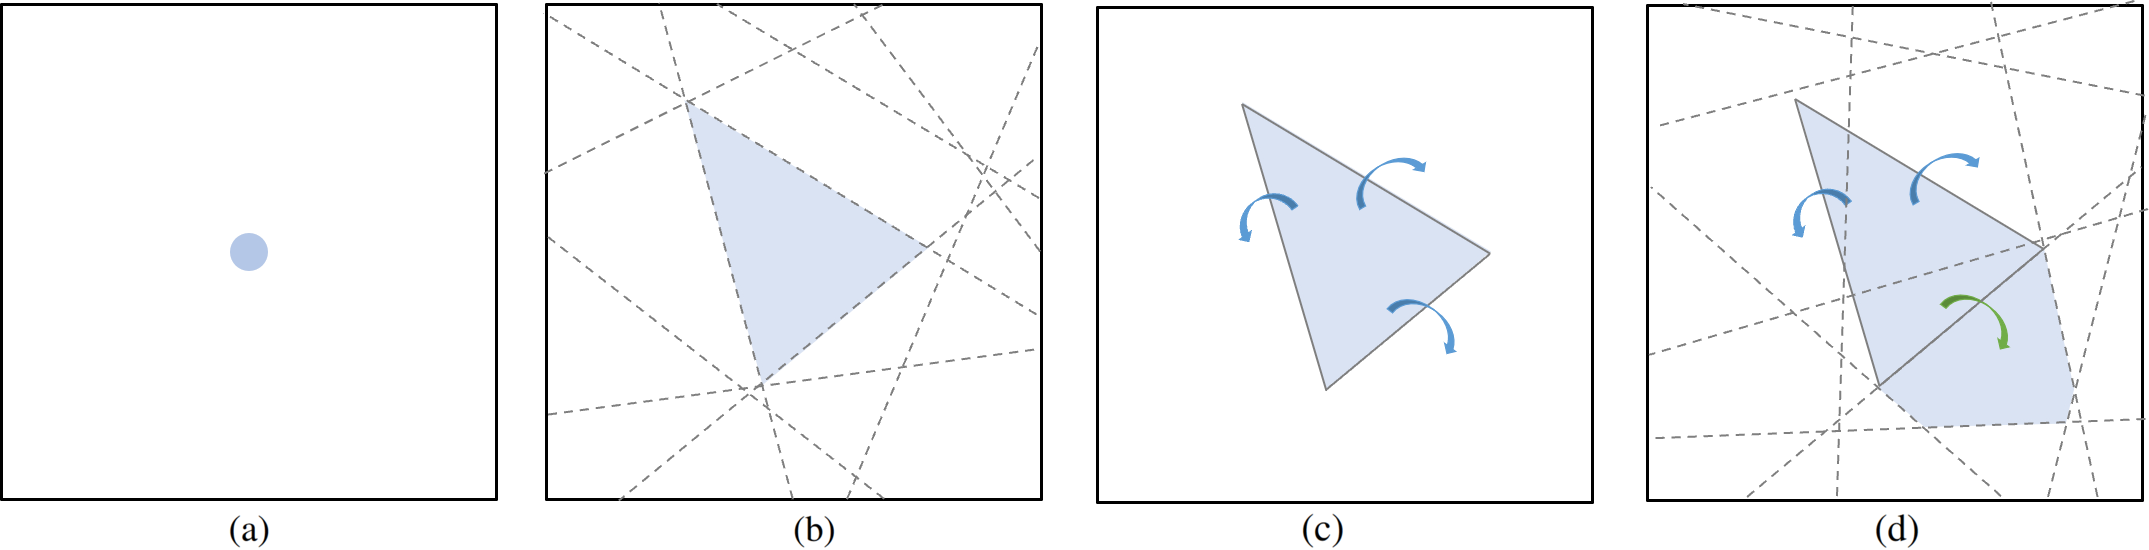
\includegraphics[width=\textwidth]{figs/rpm_fig1.png}
%     \centering
%     \caption{When transitioning from region $P_k$ to region $P_{k'}$, some neuron activations must flip to ensure their associated halfspace constraints (as given by (REF)) are valid for $P_{k'}$. In (a), two neighboring regions $P_k$ and $P_{k'}$ are shown. Constraint $1$ is the neighbor constraint $\ba_\eta^\top \bx = b_\eta$ and is shared by both regions. Constraint $2$ is different in $P_k$ and $P_{k'}$, but induced by the same neuron. We know from (REF) that only those neurons whose associated halfspace constraints in $P_k$ are scalar multiples of the neighbor constraint may need to flipped, and that in $P_{k'}$ their updated halfspace constraints will remain scalar multiples of the neighbor constraint. To flip the correct neuron activations, Algorithm REF iterates through each neuron and initially assumes each activation is the same in $P_{k'}$ as it was in $P_k$. From this assumed activation, if a neuron's constraint is a scalar multiple of the neighbor constraint then we check whether it is a feasible constraint for $P_{k'}$. Given the neighbor constraint $\ba_\eta^\top \bx \le b_\eta$ shown in blue, (b) and (e) illustrate feasible constraints while (c) and (d) do not (and therefore require the activation to be flipped). Finally, it is possible for a candidate neuron's constraint to be $\mathbf{0}^\top \bx \le b$, in which case it is feasible if $b \ge 0$ and flipped otherwise. These situations are the basis for the neuron activation flipping rules in Algorithm REF.
%     % \textcolor{black}{Mac: This is too confusing to be understood by the reader, and it's not referred to enough in the text. We should really leverage this figure in the explanation to tell the story of the flipping rules.} The activation of a neuron in $P_k$ defines a nonlinear constraint $\mathbf{a}(\bx)^\top \bx \le b(\bx)$ which may remain valid in $P_{k'}$, or may need to be flipped. Type 3 neurons need not be flipped, while Type 1 ((a)-(c)) and Type 2 ((d)-(f)) neurons may need to be flipped. Let $\mathbf{a}(\bx)^\top \bx < b(\bx)$ be shown in green, $\mathbf{a}(\bx)^\top \bx > b(\bx)$ in red, and the special case of $\mathbf{a}(\bx) = \mathbf{0}$ in blue. To determine a neuron activation in $P'$, we first determine which scenario ((a)-(f)) applies. Clearly, for the cases illustrated by (a) and (d), the neuron activation must be flipped to ensure it defines a valid constraint in $P_{k'}$. However, for the remaining scenarios, the rules for flipping neuron activations are more nuanced. A full discussion of the neuron flipping rules is given in the Appendix.
%     }
%     \label{fig:constraints}
% \end{figure*}



Building on Algorithms \ref{Algo:essential hrep} \& \ref{Algo:neighbor_ap}, we now define our main algorithm, Reachable Polyhedral Marching (RPM) in Algorithm \ref{Algo:cell_enumeration} for explicitly enumerating all polyhedra in the input space of a ReLU network, resulting in the explicit PWA representation. 
First we start with a polyhedral set of inputs we would like to enumerate affine regions over.
This set of inputs can also be $\mathbb{R}^n$, but in most applications it makes sense to consider a bounded set of inputs.
Then, we find an initial point within the input set and evaluate the network to find the activation pattern. 
% Note, this initial point should lie in the interior of a polyhedral region, not on the boundary. 
From this, the essential H-representation is found using Algorithm \ref{Algo:essential hrep}. 
For each essential constraint we generate a neighboring activation pattern using Algorithm \ref{Algo:neighbor_ap}. 
The process then repeats with each new neighboring activation pattern being added to a working set. 
For a given starting polyhedron each neighbor polyhedron is enumerated, and since all polyhedra are connected via neighbors, Algorithm \ref{Algo:cell_enumeration} is guaranteed to enumerate every polyhedron in the input space. 
Figure \ref{fig:alg_steps} illustrates the steps of RPM and Figure \ref{fig:cell_enum} shows the result of applying Algorithm \ref{Algo:cell_enumeration} to a ReLU network trained to model a quadratic function.

The bulk of the computation for Algorithm \ref{Algo:cell_enumeration} is dedicated to solving the LPs needed to retrieve the essential H-representation for each polyhedron (Algorithm \ref{Algo:essential hrep}).
In the worst case, for each polyhedron in the input space, Algorithm \ref{Algo:cell_enumeration} solves an LP for each neuron in the network. 
As noted in Section \ref{sec:relu_networks}, the number of polyhedra for the algorithm to explore scales according to $\mathcal{O}(N^n)$ where $N$ is the number of neurons and $n$ is the dimension of the input space.
Thus, in the worst case, the number of LPs solved by the algorithm scales according to $\mathcal{O}(N^{2n})$.
This exponential complexity in the input dimension is unsurprising and is inherent to the exact analysis of ReLU neural networks \cite{reluplex}.


\begin{algorithm}
\SetAlgoLined
\DontPrintSemicolon
 \KwIn{$\lambda_{0}$, $\bTheta$}
 \KwOut{Explicit PWA representation}
 PWA = $\emptyset$;  visited = $\emptyset$ \\
 working set = \{$\lambda_0$\} \\
 \While{$\text{\upshape working set} \neq \emptyset$}{
 $\lambda_k \leftarrow$ pop next $\lambda$ off working set \\
 $\bA_k, \bb_k \leftarrow$ Algorithm \ref{Algo:essential hrep} \algorithmiccomment{Retrieve essential H-rep} \\
 $\mathbf{C}_k,\ \mathbf{d}_k \leftarrow$ (\ref{eq:CdDef}) \algorithmiccomment{Retrieve affine map} \\
 push ($\bA_k, \bb_k, \bC_k, \bd_k$) onto PWA \\
 \For(\algorithmiccomment{For each neighbor}){$\mathbf{a}_{k,i}, b_{k,i} \in \bA_k, \bb_k$}{
 $\lambda_{k'} \leftarrow$ Algorithm \ref{Algo:neighbor_ap} \algorithmiccomment{$\ba_\eta, b_\eta = \ba_{k,i}, b_{k,i}$} \\
 \If{$\lambda_{k'} \notin \text{\upshape visited} \cup \text{\upshape working set}$}{
 push $\lambda_{k'}$ onto working set \\
 }
 }
 push $\lambda_k$ onto visited\\
 }
 \Return{\text{\upshape PWA}}
 \caption{Reachable Polyhedral Marching}
 \label{Algo:cell_enumeration}
\end{algorithm}